\section*{Implementation}

\subsection*{Development Environment} 
The development of Cuteserver was primarily accomplished through pair programming. We held regular meetings where we shared our terminals using a shell sharing tool called \textbf{sshx} \footnote{SSHX. https://sshx.io/}. This tool was particularly effective for collaboration since we both used \textbf{Neovim} as our code editor. \\
 
Initially, we used \textbf{Makefiles} to build the source code, but this approach was inefficient due to frequent adjustments. As the project grew more complex, we decided to use \textbf{CMake} for more efficient project building and file generation. \\

Our implementation strategy for the web server was iterative, starting with small, manageable tasks and progressively tackling more complex ones. We regularly tested the code by running it with different inputs to ensure functionality.

\subsection*{Project Structure} 
We structured our code into modules, each handling a task or describing a logical "unit". In the main module the server socket is set up and incoming TCP connections are handled through a threadpool. When a new request is received, a thread starts serving the incoming request. Our implementation supports Keep-Alive Headers. Per default a "keep-alive"-Connection is assumed, so multiple responses can be sent over one TCP connection. (See Results). To prevent too many idle connections, a timeout of 5 Seconds is set. 
%NOTE: Server waits for 7s though.  

\subsection*{Static File Requests}
Each incoming request is parsed into request line, headers and body, and saved in a struct called request\_info. We differentiate between static (GET or HEAD) and dynamic (GET or POST) requests. 
For static requests, we access the file to receive metadata such as content length and type. For HEAD-Requests only the Headers are sent, for GET-Requests the file is also sent.  

\subsection*{CGI}
Dynamic Request are handled with CGI. This means the incoming request is parsed, then passed to the CGI handler which creates a new process running the corresponding cgi script. The CGI Protocol defines "meta-variables" \footnote{RFC 3875. CGI Specification. Section 4.1 Request Meta-Variables. https://datatracker.ietf.org/doc/html/rfc3875#section-4.1} which have to be passed from server to CGI script using environment variables. \\

The CGI process is started using the \textbf{execve} function, allowing us to pass the environment variables as an argument. Additional data has to be passed to the child process through standard in/output. \footnote{Mapping UNIX pipe descriptors to stdin and stdout. http://www.unixwiz.net/techtips/remap-pipe-fds.html}
Communication between cgi process and server (parent process) is enabled through pipes. A pair of pipe descriptors is created before the child process is forked. Then, the child's descriptors are redirected to standard input and standard output \footnote{Pipes. http://www.fmc-modeling.org/category/projects/apache/amp/A_4_Pipes.html} (See Figure 3).

\begin{figure}[h]
	\centering
	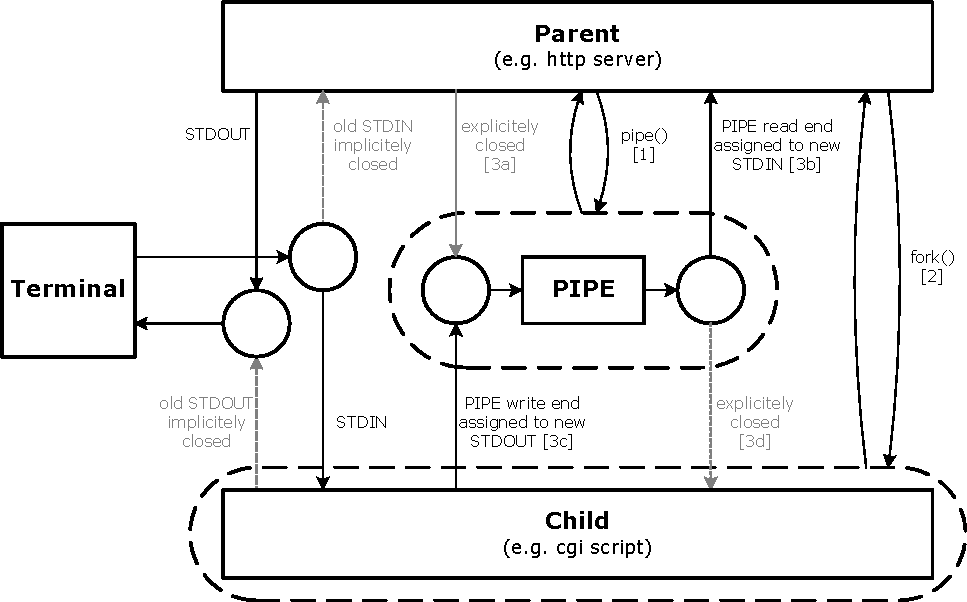
\includegraphics[width=0.7\textwidth]{figures/Pipes_BD.pdf}
	\caption{Pipe Redirection}
    \floatfoot{\small Source: http://www.fmc-modeling.org/category/projects/apache/amp/A_4_Pipes.html}
\end{figure}

\subsection*{Server Configuration}
From the beginning, we aimed for our web server to support hosting multiple resources connected to different domain names. To achieve this multidomain support, we needed to make the web server configurable. To ensure user-friendly configuration, we used \textbf{TOML} files. The web server parses a configuration file listing all resources and their locations for the server to serve. Additionally, users can specify resource-independent settings, such as the number of active worker threads and log storage locations. We also provide a command line interface where users can specify the TCP address and the path to the configuration file.

\subsection*{Example Application}
% TODO: synchronization 

We had several web applications to test our web server. Initially, we used simple HTML files and gradually added more complex ones. Eventually, we developed a more sophisticated application using the React framework for the front end. This application is a simple chat app that makes POST requests when users submit chat messages. These POST requests are handled by our backend service, which stores the chat messages in a JSON file and sends the JSON data to clients. We initially wrote this service using the Flask framework in Python to test if interpreted languages could work as CGI scripts. While this worked, we later translated the backend Python script to a C script to achieve faster response times by running compiled executables. 

\begin{figure}[h]
	\centering
	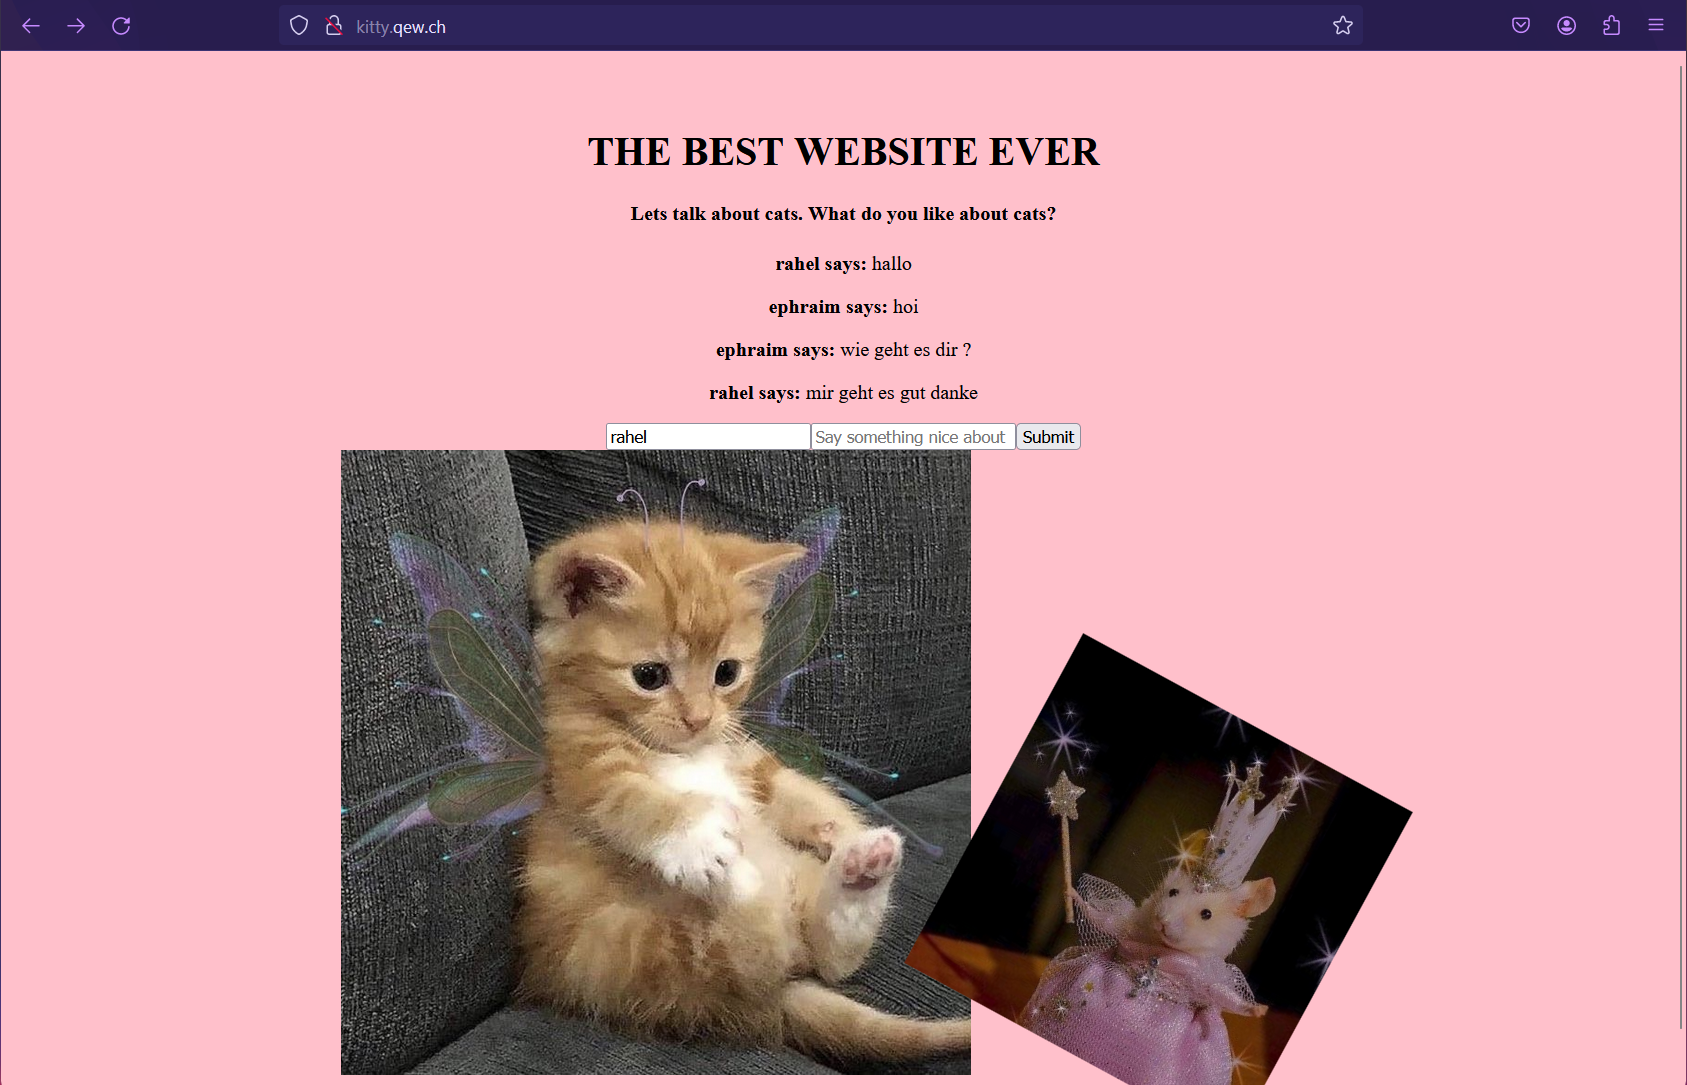
\includegraphics[width=\textwidth]{figures/screenshot_ex_app.png}
    \caption{Our Example Application}
\end{figure}

\subsection*{Containerization}
We decided to containerize our application for two main reasons. Initially, we used chroot jails to sandbox our application, i.e., a mechanism that isolates a process and its children from the rest of the system by changing their apparent root directory to a specified path. This approach worked until we implemented CGI support, which required the web server to start new processes with the necessary libraries for the CGI scripts. Manually copying those dependencies into the chroot jail would have been too laborious. Docker containers offered an easier solution by securely sandboxing execution and including dependencies. Additionally, Dockerfiles enabled us to automate the building of the web server and the example application, making it easy to use and run. We used multistage builds, first creating containers for building and then copying only the necessary files to the final containers. Multistage build reduced the container size from 1.2 GB to approximately 200 MB. This process enhanced our understanding of containerization.
